%% LaTeX2e class for seminar theses
%% seminar.tex
%% 
%% Karlsruhe Institute of Technology
%% Institute for Program Structures and Data Organization
%% Chair for Software Design and Quality (SDQ)
%%
%% Dr.-Ing. Erik Burger
%% burger@kit.edu
%%
%% Version 1.0.1, 2018-04-16

%% Available page modes: oneside, twoside
%% Available languages: english, ngerman
%% Available modes: draft, final (see README)
\documentclass[oneside, english, final]{sdqseminar}
%% ---------------------------------
%% | Information about the thesis  |
%% ---------------------------------

%% Name of the author
\author{Christian  Oder}

%% Title (and possibly subtitle) of the thesis
\title{Android custom ROM development}

%% Type of the thesis 
% \thesistype{Seminar Thesis}

%% Change the institute here, ``IPD'' is default
% \myinstitute{Institute for \dots}

\settitle

%% --------------------------------
%% | Settings for word separation |
%% --------------------------------

%% Describe separation hints here.
%% For more details, see 
%% http://en.wikibooks.org/wiki/LaTeX/Text_Formatting#Hyphenation
\hyphenation{
% me-ta-mo-del
}

%% --------------------------------
%% | Glossary                     |
%% --------------------------------

\makenoidxglossaries
\newacronym{ac:aosp}{AOSP}{\gls{gls:aosp}}
\newglossaryentry{gls:aosp}
{ name=Android Open Source Project,
	description={Android is an open source operating system for mobile devices and a corresponding open source project led by Google. This site and the Android Open Source Project (AOSP) repository offer the information and source code needed to create custom variants of the Android OS, port devices and accessories to the Android platform, and ensure devices meet the compatibility requirements that keep the Android ecosystem a healthy and stable environment for millions of users \citep{web:aosp}}}
\newglossaryentry{gls:carbon}
{ name=CarbonROM,
	description={CarbonROM is an aftermarket firmware based on the \gls{gls:aosp} created with the purpose of adding versatility and customization to stock Android. Stability is the highest priority. Their vision is to be the best alternative to a stock operating system on an users device \citep{web:carbon}}}
\newglossaryentry{gls:lineage}
{ name=LineageOS,
	description={A free and open-source operating system for various devices, based on the Android mobile platform. The biggest of it's kind with almost 1.8 million active users as of January 2019 \citep{web:lineage}}}
\newglossaryentry{gls:omnirom}
{ name=OmniROM,
	description={OmniROM is our Android custom ROM variant, feature-packed but always with stability as number one priority in mind.
Based on the \gls{gls:aosp} (\acrshort{ac:aosp}) and enriched by their developers with lots of custom enhancements, OmniROM has set out to give their users a great Android experience on their mobile \citep{web:omnirom}}}
\newglossaryentry{gls:timekeep}
{ name=timekeep,
	description={TimeKeep is a small utility to keep track of time and date since the RTC driver on Qualcomm chipset is read-only. It originates from \acrshort{ac:sodp} \citep{web:sodp}}}
\newglossaryentry{gls:z3}
{ name=Sony Xperia Z3,
	description={A Smartphone released in 09/2014 by Sony Mobile.
	Featuring a Qualcomm Snapdragon S801 and 3GB of RAM along with a Full HD screen it was considered a flagship device upon release and is still more than powerful enough to handle modern Software \citep{web:z3}}}
\newacronym{ac:z3}{Xperia Z3}{\gls{gls:z3}}
\newglossaryentry{gls:s9}
{ name=Samsung Galaxy S9,
	description={A Smartphone released in 02/2018 by Samsung Mobile.
	Featuring a Samsung Exynos 9810 Octa Core CPU and 4GB of RAM along with a 1440x2960 screen it is considered a modern day flagship device and is the newest device available from Samsung. Usually a prime example of fast Software updates \citep{web:s9}}}
\newacronym{ac:selinux}{SELinux}{\gls{gls:selinux}}
\newglossaryentry{gls:selinux}
{ name=Security-Enhanced Linux,
	description={Security-Enhanced Linux (SELinux) is a Linux kernel security module that provides a mechanism for supporting access control security policies, including mandatory access controls (MAC) \citep{web:selinux}.}}
\newacronym{ac:hal}{HAL}{\gls{gls:hal}}
\newglossaryentry{gls:hal}
{ name=Hardware Abstraction Layer,
	description={The Hardware Abstraction Layer is a software subsystem for UNIX-like operating systems providing hardware abstraction. Hardware abstractions are sets of routines in software that emulate some platform-specific details, giving programs direct access to the hardware resources \citep{web:HALWikipedia}}}
\newglossaryentry{gls:wpas}
{ name=wpa\_supplicant,
	description={wpa\_supplicant is a cross-platform supplicant with support for WEP, WPA and WPA2 (IEEE 802.11i). It is suitable for desktops, laptops and embedded systems. It is the IEEE 802.1X/WPA component that is used in the client stations. It implements key negotiation with a WPA authenticator and it controls the roaming and IEEE 802.11 authentication/association of the wireless driver \citep{web:ArchlinuxWikiWPASupplicant}}}
\newacronym{ac:sodp}{SODP}{\gls{gls:sodp}}
\newglossaryentry{gls:sodp}
{ name=Sony Open Device Program,
	description={The Sony Open Device Program is an Sony introduced Program where they provide binaries and device sources as well as changes needed to build the \gls{gls:aosp} for their devices \citep{web:sodp}}}


%% --------------------------------
%% | Bibliography                 |
%% --------------------------------

\bibliographystyle{abbrvnat}

%% --------------------------------
%% | Hypenation Protection        |
%% --------------------------------
\hyphenation{Android}

%% ====================================
%% ====================================
%% ||                                ||
%% || Beginning of the main document ||
%% ||                                ||
%% ====================================
%% ====================================
\begin{document}

%% Set PDF metadata
\setpdf

%% Set the title
\maketitle

%% ----------------
%% |   Abstract   |
%% ----------------
 
%% The text is included from the following files:
%% - sections/abstract

\begin{abstract}
%% LaTeX2e class for seminar theses
%% sections/abstract_en.tex
%% 
%% Karlsruhe Institute of Technology
%% Institute for Program Structures and Data Organization
%% Chair for Software Design and Quality (SDQ)
%%
%% Dr.-Ing. Erik Burger
%% burger@kit.edu
%%
%% Version 1.0, 2018-04-16

On how to bring the latest Android to some of the oldest Smartphones
\end{abstract}

%% -----------------
%% |   Main part   |
%% -----------------

%% LaTeX2e class for seminar theses
%% sections/content.tex
%% 
%% Karlsruhe Institute of Technology
%% Institute for Program Structures and Data Organization
%% Chair for Software Design and Quality (SDQ)
%%
%% Dr.-Ing. Erik Burger
%% burger@kit.edu
%%
%% Version 1.0, 2018-04-16

\section{Introduction}
\label{ch:Introduction}

The custom ROM scene, especially for older devices is growing continuously. In times, where security vulnerabilities are discovered on a daily basis, software updates are highly important. Due to planned obsolescence and the lack of intrests from OEMs many Android devices are highly outdated and exploitable by most of the common security flaws.

For example, the 2014 \gls{gls:z3}'s last update of Android 6.0 included Security Patches from early 2016, which is already above the common standards on devices released in that timeframe.
\defcitealias{web:dirtycow}{Dirty Cow}
However, that still leaves the device with vulnerabilities like \citetalias{web:dirtycow}, a fairly high security risk.

In order to circumvent this, and thanks to Android being Open Source users can install aftermarket firmware on their device, the so called custom ROM\footnote{The Term ROM originates from old devices that used to have a Read Only Memory for their system partition}. Hence it's possible to always have the latest Security Patches on an fairly old phone. This can't be said about even some of the most recent devices. For example, the \gls{gls:s9} just recently got the Update to Android 9 near Christmas of December 2018\footnote{https://www.netzwelt.de/samsung-galaxy-s9/168265-galaxy-s9-plus-stand-android-90-pie-rollouts-ueberblick.html} whereas, thanks to custom ROMs, the \acrshort{ac:z3} got Android 9.0 back in the end of October, and currently runs the (as per time of writing) 3 days ago released January Security Patches\footnote{\label{jan_asb}https://source.android.com/security/bulletin/2019-01-01} as shown in Figure~\ref{fig:z3_january_asb} below.

\newpage

\begin{figure}
\centering
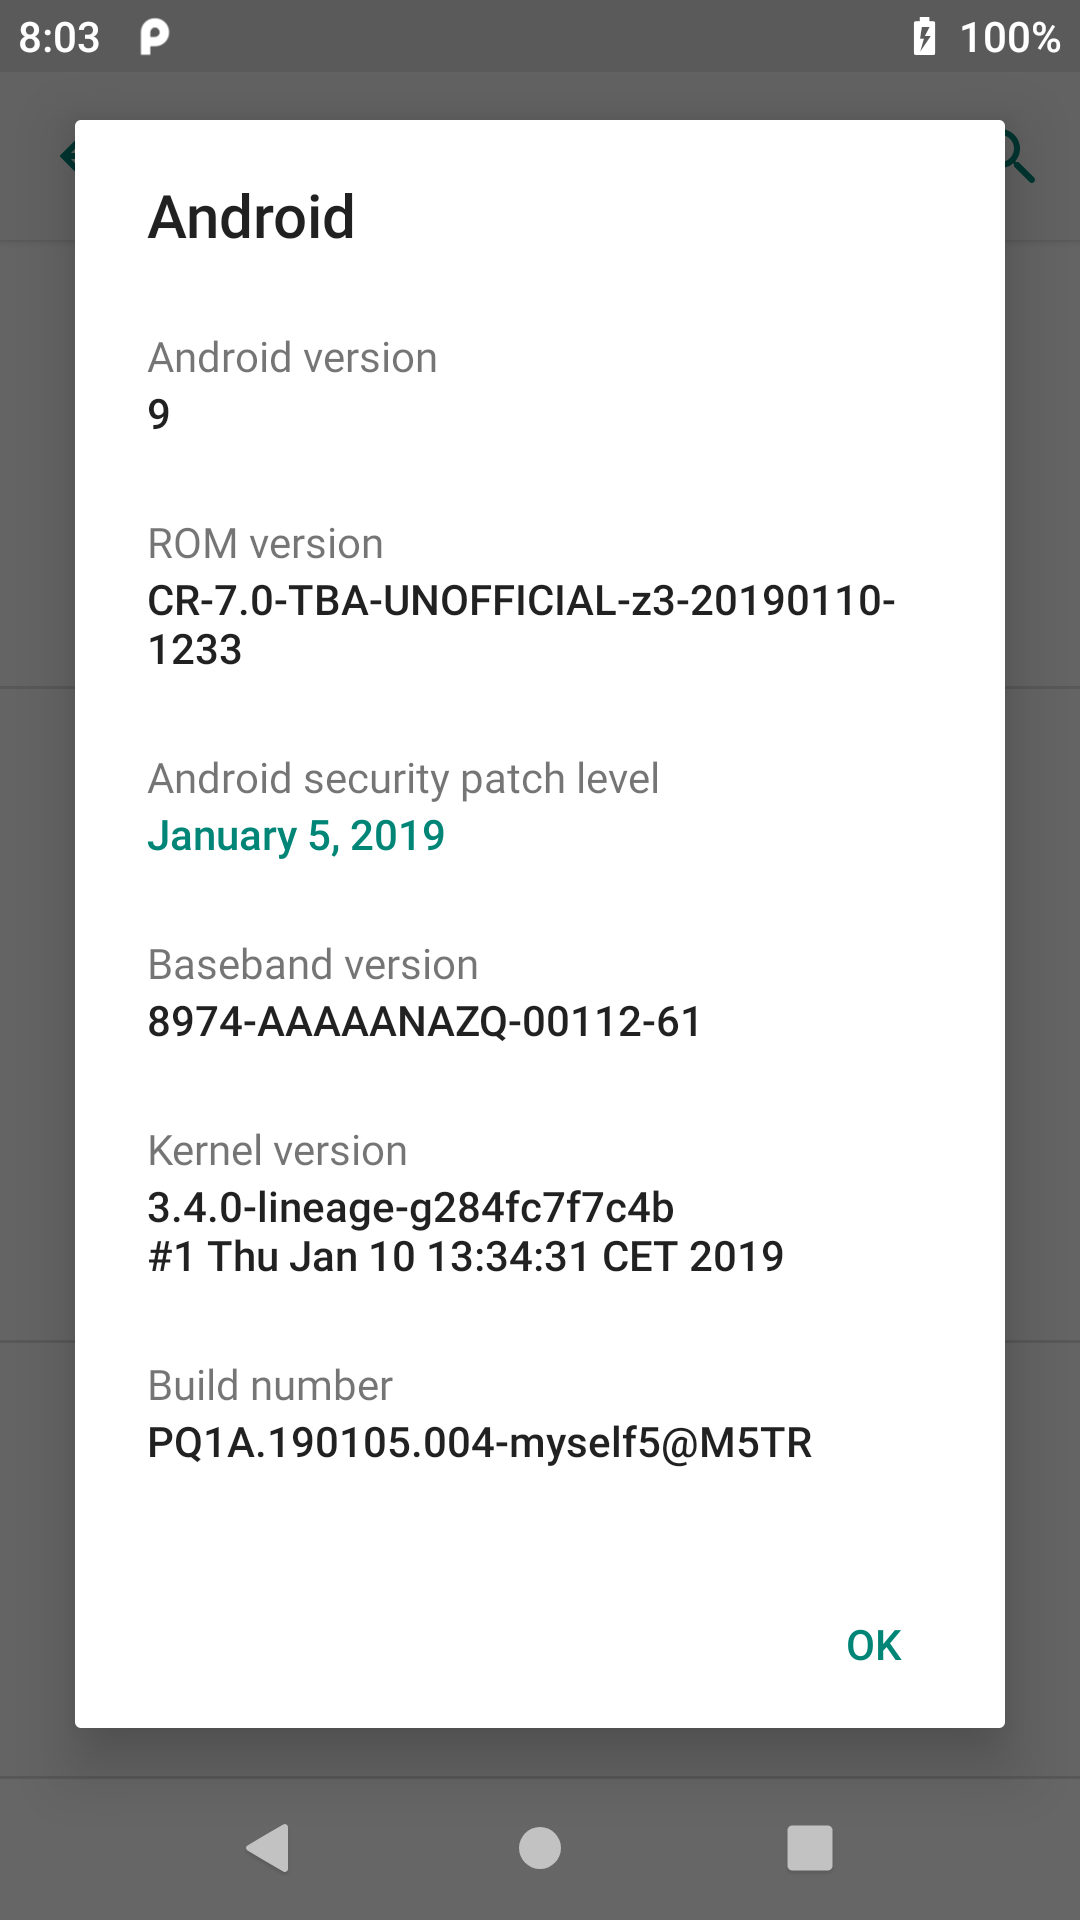
\includegraphics[width=7cm]{images/z3_january_asb}
\caption{\gls{gls:z3} running ~Android 9 with January Security Patches}
\label{fig:z3_january_asb}
\end{figure}

On top of that, the variety of custom ROMs available allows an user to choose between different system sided features that might not be part of the original firmware, which, besides the security patches, is a reason to go custom for many.
In order to provide these aftermarket firmwares each device requires it's own sources, which in addition require certain updates every Major Android revision. These will be explained in detail on the example of the \gls{gls:z3} on \gls{gls:carbon}.

\newpage
%% LaTeX2e class for seminar theses
%% sections/content.tex
%% 
%% Karlsruhe Institute of Technology
%% Institute for Program Structures and Data Organization
%% Chair for Software Design and Quality (SDQ)
%%
%% Dr.-Ing. Erik Burger
%% burger@kit.edu
%%
%% Version 1.0, 2018-04-16

The general procedure can be seperated in three steps:
\begin{itemize}
	\item{\nameref{ch:GettingItToBuild}}
	\item{\nameref{ch:BootingTheDevice}}
	\item{\nameref{ch:FixingFeatures}}
\end{itemize}

\section{Getting it to build}
\label{ch:GettingItToBuild}

The first step is to adapt the device sources to changes inside the Android framework, so that we can successfully compile a ROM for said device.
On the \gls{gls:z3} the below mentioned steps were required. The responding commits are below each subsection.

\subsection{Removing old configs}

The HWUI config imported in the device tree contained only obsolete configs. It therefore is no longer existent and we need to remove the inclusion.

\href{https://github.com/CarbonROM/android_device_sony_z3/commit/5e0b81ac20be8adcb7e7f42ba431175c0d56c917}{https://github.com/\\CarbonROM/android\_device\_sony\_z3/commit/5e0b81ac20be8adcb7e7f42ba431175c0d56c917}

\subsection{Adjusting the init library}
The init library is, as the name suggests, responsible for preparing and starting the system.
The init is extended by the devicetree in order to handle device specific requirements.
Due to method changes in Pie, we need to adjust our init extension.

\url{https://review.carbonrom.org/c/CarbonROM/android_device_sony_shinano-common/+/8106}

\subsection{Updating the libshim}

Shims are libraries to replace code in other libraries. Upon boot, the bionic libraries load those shim libs over existing libraries and replace certain method calls.
That is neccessary when a method signature changes across Android releases (like it would on Android 9 with the binaries from Android 6.0) or when a method needs to be replaced (like working around camera DRM limitations).

On the \gls{gls:z3} we needed to update the signal.h shim based on the Android 9 signal header to handle method and structural changes.

\url{https://review.carbonrom.org/c/CarbonROM/android_device_sony_msm8974-common/+/8088}

\subsection{Handling basic changes in SELinux}

\acrshort{ac:selinux} rules and definitions usually change across the releases, so we need to adjust ours with some basic changes. Denials will be solved later on. In theory \acrshort{ac:selinux} could be disabled, although it's better practice to solve the basic issues beforehand as some services require \acrshort{ac:selinux} domains in order to work. On some devices that could prevent the device from booting successfully, in our case we know that the SIM Services and therefore mobile radio would have been broken.
As we're dealing with a legacy device, we're now using the Qualcomm provided legacy \acrshort{ac:selinux} rules.

Nonetheless, until we we reach \ref{sub:selinux_denials}, we're going to operate the system in \acrshort{ac:selinux} Permissive mode. That mode logs when there would be a denial so that it can be fixed later on, but grants access for the time being.

\url{https://review.carbonrom.org/c/CarbonROM/android_device_sony_shinano-common/+/8107}\\
\url{https://review.carbonrom.org/c/CarbonROM/android_device_sony_msm8974-common/+/8113}

\subsection{Kernel changes}

On some Android revisions there are multiple Kernel changes required in order to build or boot. For example on Android 8.0, the Kernel required the introduction of Kernel feature to handle the new \gls{gls:hal}.

On Android 9, only small changes have been done, which is why we only require small header changes.

\url{https://review.carbonrom.org/c/CarbonROM/android_kernel_sony_msm8974/+/8098}\\
\url{https://review.carbonrom.org/c/CarbonROM/android_kernel_sony_msm8974/+/8097}

(the latter should be considered a Hack for now and will be replaced by the original commits with proper authorship)

\subsection{Fixing the FM driver}
\label{sub:fixing_fm}

The FM driver, responsible for the FM Radio handling is not made by Google. The project it originates from is no longer updated, so the community needs to take care of that.
Android 9 introduced a lot stricter global C-flags so the build would error out on certain C warning, like an unused variable.

This is solved be either solving the warnings, like removing an unused variable, or reintroducing the C flags for the troublesome code.

\href{https://github.com/CarbonBeta/android_hardware_broadcom_fm/commit/7ccedbcea03e93de47d4d17034436f3ed5b5f671}{https://github.com/\\CarbonBeta/android\_hardware\_broadcom\_fm/commit/7ccedbcea03e93de47d4d17034436f3ed5b5f671}

\section{Booting the device}
\label{ch:BootingTheDevice}
Just because the ROM now successfully compiles, it doesn't mean that it boots. Very often, there are additional commits required to get the device booting, or to prevent it from crashing right away.

Thankfully, that was not the case on the \gls{gls:z3}, but as we were expecting this to happen we already made some pretaration.
Due to changes in the USB \acrshort{ac:hal} we now need to set an USB compat mode for USB debugging to work.
We do that by setting \texttt{sys.usb.ffs.aio\_compat} to \texttt{1} at boot and introducing our own basic USB \acrshort{ac:hal}.

\url{https://review.carbonrom.org/c/CarbonROM/android_device_sony_shinano-common/+/8136}\\
\url{https://review.carbonrom.org/c/CarbonROM/android_device_sony_msm8974-common/+/8092}\\
\url{https://review.carbonrom.org/c/CarbonROM/android_device_sony_msm8974-common/+/8093}\\
\url{https://review.carbonrom.org/c/CarbonROM/android_device_sony_msm8974-common/+/8095}

\section{Fixing broken features}
\label{ch:FixingFeatures}

Now that our phone boots, we move on to checking what is working and what is not, so that we can solve that.

\subsection{Fixing WiFi}

From other devices we roughly know what kind of changes are needed to fix which issue. In terms of WiFi, we know that we have a Broadcom WiFi and Bluetooth chip.
What we do, is increasing the revisions of the \gls{gls:wpas} and the WiFi \acrshort{ac:hal}.
On top of that, the flags passed to the \gls{gls:wpas} service need to be adjusted to deal with changes in Android 9.

For example we need to move the \gls{gls:wpas} control socket to a new path, as Android 9 doesn't allow sockets to be in \texttt{data/misc/wifi/sockets}.

Instead, they have to be in \texttt{/data/vendor/wifi/wpa/sockets} now. These changes were common on almost any Android device getting updated to Android 9.

\url{https://review.carbonrom.org/c/CarbonROM/android_device_sony_shinano-common/+/8082}\\
\url{https://review.carbonrom.org/c/CarbonROM/android_device_sony_shinano-common/+/8084}\\
\url{https://review.carbonrom.org/c/CarbonROM/android_device_sony_shinano-common/+/8085}\\
\url{https://review.carbonrom.org/c/CarbonROM/android_device_sony_shinano-common/+/8086}\\
\url{https://review.carbonrom.org/c/CarbonROM/android_device_sony_msm8974-common/+/8089}\\
\url{https://review.carbonrom.org/c/CarbonROM/android_device_sony_msm8974-common/+/8090}\\
\url{https://review.carbonrom.org/c/CarbonROM/android_device_sony_msm8974-common/+/8091}

In addition, we require small changes to the \gls{gls:aosp} (\acrshort{ac:aosp}) repository. Instead of maintaining our own fork for that, we're going to use the \texttt{hardware/broadcom/wifi} repository from \gls{gls:lineage}.

\url{https://review.carbonrom.org/c/CarbonROM/android/+/8109}

\subsection{Solving the Bluetooth by getting back the MAC Address}

Bluetooth was rather tricky. We already knew that it's required to change move the socket and therefore that it's required to create the folder structure for that, but even then bluetooth would not work. The reason behind that, was that it failed to read the bluetooth address from the socket in \texttt{/data/vendor/bluetooth/bluetooth\_bdaddr}.

That's caused by the the way MAC address handling is done on Sony devices. The address is stored on a seperate partition, the \texttt{TA} Partition.
To read from that address, we use \texttt{macaddrsetup}. The \texttt{macaddrsetup} we used reads the address from \texttt{TA}, and writes it to the socket in \texttt{/data/misc/bluetooth/bluetooth\_bdaddr}. That socket is wrong for Android 9. However, \acrshort{ac:sodp} already updated \texttt{macaddrsetup} to write to the correct socket\footnote{\url{https://github.com/sonyxperiadev/macaddrsetup/commit/a7416d68697ae60f5f5fcd53db5ead7081a06bc6}}. So the issue has been solved by using the updated \texttt{macaddrsetup}.

As pointed out by a \gls{gls:lineage} developer later on, the \texttt{} repository from \ref{sub:fixing_fm} is required for bluetooth too. Removing that while thinking that the FM radio would't work due to the lack of App and framework support would not work anyways he later on quickly regretted that decision.

\url{https://review.carbonrom.org/c/CarbonROM/android/+/8142}\\
\url{https://review.carbonrom.org/c/CarbonROM/android_device_sony_msm8974-common/+/8148}

Additionally, it was necessary to add changes to \texttt{hardware/broadcom/libbt}. As \gls{gls:lineage} has all those changes, we use their repository.

\url{https://review.carbonrom.org/c/CarbonROM/android/+/8142}

\subsection{Using a prebuilt NFC \acrshort{ac:hal}}

The NXP Semiconductors PN547 chip used in the \acrshort{ac:z3} is no longer properly supported by the \gls{gls:aosp}.
We therefore no longer compile the drivers but instead use a prebuilt solution with binaries built with Android 8.0.

That means we remove the package inclusions of the NFC binaries in the device tree and add the prebuilt binaries to the \texttt{vendor/sony} repository that contains the proprietary binaries.

\url{https://review.carbonrom.org/c/CarbonROM/android_device_sony_msm8974-common/+/8134}\\
\url{https://review.carbonrom.org/c/CarbonROM/android_device_sony_shinano-common/+/8137}\\
\href{https://github.com/obsd39/proprietary_vendor_sony/commit/9708b725aaef8634ad345bebbf3e36ed6d07b27d}{https://github.com/\\obsd39/proprietary\_vendor\_sony/commit/9708b725aaef8634ad345bebbf3e36ed6d07b27d}

It's also required to adjust the NFC config that defines supported features by removing the feature configs that are unsupported in Android 9 and by renaming the config so that it gets picked up by the system.

\url{https://review.carbonrom.org/c/CarbonROM/android_device_sony_z3/+/8080}

\subsection{Fixing the Camera after restarts}
On the first boot, the camera would work fine. However, after a reboot the system is not granting access to the camera because the calling process is the \texttt{mediaserver}.
By default, Android would only allow the \texttt{cameraserver} to communicate with the camera. This commit conditionally allows the camera to be access by the \texttt{mediaserver} too, so we add that to the framework

\url{https://review.carbonrom.org/c/CarbonROM/android_frameworks_base/+/8160}

and enable it in the devicetree.

\url{https://review.carbonrom.org/#/c/CarbonROM/android_device_sony_msm8974-common/+/8209}

\subsection{Solving media playback issues}
With outdated graphics drivers as the \acrshort{ac:z3} has, the gralloc buffer requires certain usage bits that are no longer allowed in Android 9.

The gralloc handling has therefore been extended to allow accepting a custom set of gralloc flags

\href{https://github.com/CarbonROM/android_frameworks_native/commit/50a0f37295047560801e9de4beae91704c60b256}{https://github.com/\\CarbonROM/android\_frameworks\_native/commit/50a0f37295047560801e9de4beae91704c60b256}

and those flags have been defined in the devicetree.

\url{https://review.carbonrom.org/c/CarbonROM/android_device_sony_msm8974-common/+/8096}

\subsection{Solving \acrshort{ac:selinux} Denials}
\label{sub:selinux_denials}
After the existing flaws have been solved, \acrshort{ac:selinux} denials should be solved so that \acrshort{ac:selinux} can bet set to run in Enforcing mode again.
\acrshort{ac:aosp} has a very detailed writeup on how to detect, handle and solve \acrshort{ac:selinux} denials\footnote{\url{https://source.android.com/security/selinux/validate}}.

A good orientation is using \texttt{audit2allow}, however common sense should be used when writing the rules. We updated our SELinux rules to adjust for Android internal changes as well as updated subsystem like the updates of \gls{gls:timekeep}.

\url{https://review.carbonrom.org/c/CarbonROM/android_device_sony_shinano-common/+/8140}\\
\url{https://review.carbonrom.org/c/CarbonROM/android_device_sony_msm8974-common/+/8114}\\
\url{https://review.carbonrom.org/c/CarbonROM/android_device_sony_msm8974-common/+/8115}\\
\url{https://review.carbonrom.org/c/CarbonROM/android_device_sony_msm8974-common/+/8116}\\
\url{https://review.carbonrom.org/c/CarbonROM/android_device_sony_msm8974-common/+/8146}

\subsection{Miscellaneous}

This section will be about the changes that were done without fixing any \enquote{apparent} issues.

We moved \texttt{tad\_static}, a binary responsible mainly for the camera, but for almost everything else on newer Sony devices to to be running as a \texttt{core} service instead of having it run in the now semi-abandoned \texttt{trimarea} context. This did not solve or cause any issues on the \acrshort{ac:z3}, however, on one of it's successors, the Sony Xperia XZ Premium and Sony Xperia XA2 this would solve a variety of issues with mobile radio and other services.

\url{https://review.carbonrom.org/c/CarbonROM/android_device_sony_shinano-common/+/8139}

We updated the power \acrshort{ac:hal} from Version \texttt{1.0} to \texttt{1.1}. The power \acrshort{ac:hal} is responsible for power management. The system would work without it, but the battery life would be greatly impacted. We also removed references to the previously used \gls{gls:lineage} power \acrshort{ac:hal}.

\url{https://review.carbonrom.org/c/CarbonROM/android_device_sony_msm8974-common/+/8108}\\
\url{https://review.carbonrom.org/c/CarbonROM/android_device_sony_msm8974-common/+/8110}

The tethering configurations have been removed in order to let Android automatically handle the upstream network

\url{https://review.carbonrom.org/c/CarbonROM/android_device_sony_msm8974-common/+/8111} 

And we updated the sources for the latest changes in the \acrshort{ac:sodp} \gls{gls:timekeep} as well as other \acrshort{ac:sodp} repositories (hosted by \gls{gls:omnirom}).

\url{https://review.carbonrom.org/c/CarbonROM/android_device_sony_shinano-common/+/8081}\\
\url{https://review.carbonrom.org/c/CarbonROM/android_device_sony_shinano-common/+/8141}\\
\url{https://review.carbonrom.org/c/CarbonROM/android_device_sony_msm8974-common/+/8148}

%% ---------------------
%% | / Example content |
%% ---------------------
\newpage
%% LaTeX2e class for seminar theses
%% sections/conclusion.tex
%% 
%% Karlsruhe Institute of Technology
%% Institute for Program Structures and Data Organization
%% Chair for Software Design and Quality (SDQ)
%%
%% Dr.-Ing. Erik Burger
%% burger@kit.edu
%%
%% Version 1.0, 2018-04-16

\section{Conclusion}
\label{ch:Conclusion}

As seen, updating a devices sources to the latest Android revision is not easy, consumes quite a bit of time, could be frustrating at times and might not always end up working 100\%.
However, the advantages of being protected from the latest security risks while not being required to buy a new device while the old one is perfectly fine for someones needs,
and therefore being able to counter planned obsolescence do, to me and many others, outweight these disadvantages and are worth the effort.

Paired with the postive feedback and happiness you're faced with as a developer, this project as well as the custom ROM scene is just a lot of fun.

I'd like to thank Arian\footnote{https://github.com/ArianK16a}, Max Weffers\footnote{https://github.com/rcstar6696} and Nikhil Punathil\footnote{https://github.com/drakonizer} as well as everyone else from the \gls{gls:carbon}\footnote{https://github.com/CarbonROM} team for their help when it was needed.
\newpage

%% --------------------------------
%% | Glossary                     |
%% --------------------------------

\printnoidxglossary
\printnoidxglossary[type=\acronymtype]

%% --------------------
%% |   Bibliography   |
%% --------------------

%% Add entry to the table of contents for the bibliography
\bibliography{seminar}

\end{document}